\section{Introduction}
\begin{frame}{Why}
\begin{itemize}
\item How to model real world objects? - Design
\item How to put forth ideas in visual manner – Communication
\item How to verify that design serves the purpose – Analysis
\item How to get it made? – Manufacturing
\end{itemize}
All of the above can happen without Computers..but\\
Better if assisted by Computers/Software \\
\bigskip
That's why : Computer Aided $\ldots$ (CAx)
\end{frame}
%------------------------------------------------------------------------------------------------------------------------------------

\begin{frame}{Classification}
\begin{itemize}
\item By dimensionality: 2D/3D
\item 2-Manifold vs Non-manifold
\item Precision: Exact/Approximate
\item What to store?
	\begin{itemize}
	\item Procedure
	\item Result
	\item Hybrid
	\end{itemize}
\end{itemize}
\end{frame}

\begin{frame}{By dimensionality}
\begin{itemize}
\item 2D model: Point, line, circular arc, planar curve
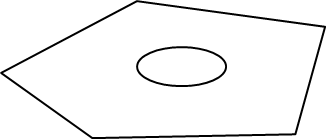
\includegraphics[scale=0.3]{images/CAD2dprofile.png}
\item 3D model
	\begin{itemize}
	\item Wire frame

	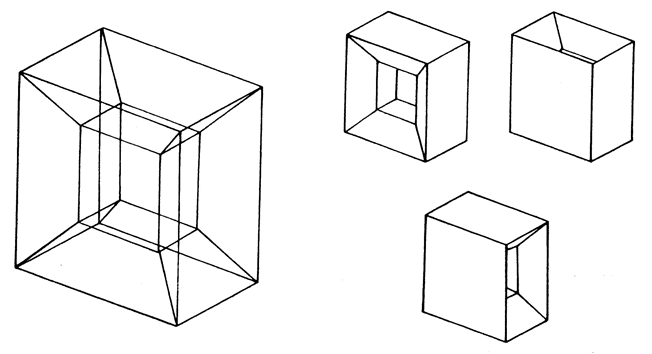
\includegraphics[scale=0.3]{images/CADWireframe.png}
	\item Surface

	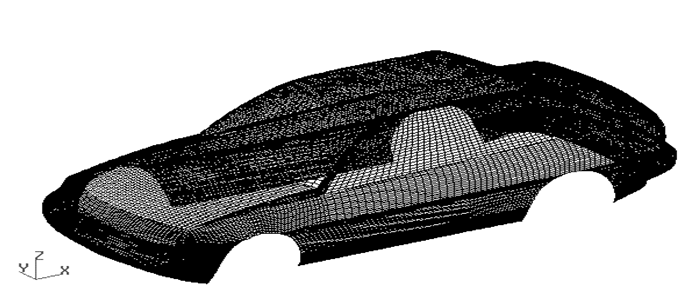
\includegraphics[scale=0.3]{images/CADSurface.png}
	\item Solid

	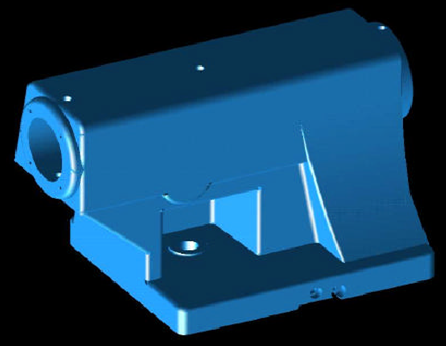
\includegraphics[scale=0.3]{images/CADSolid.png}
	\end{itemize}
\end{itemize}
\end{frame}

\begin{frame}{By Precision}
\begin{itemize}
\item Exact (?) model : Continuous/Smooth representation. Explicit / implicit / parametric curves / surfaces
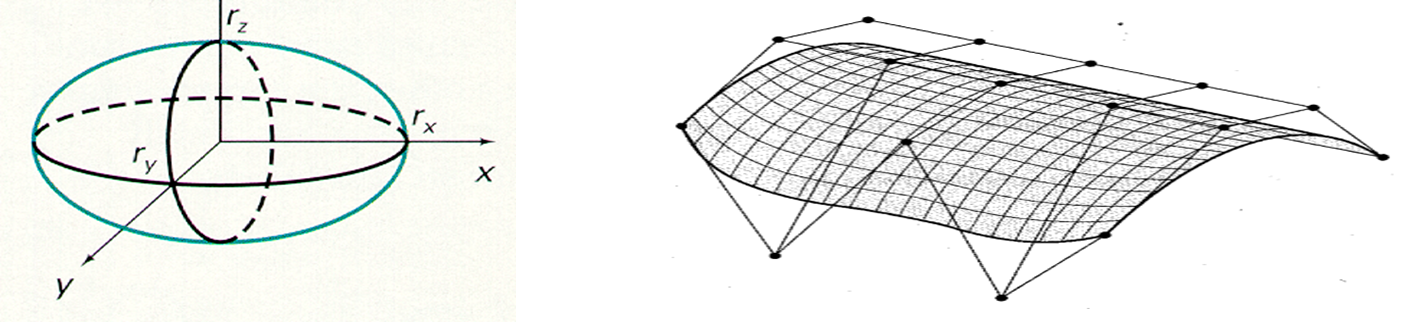
\includegraphics[scale=0.2]{images/CADExact.png}
\item Approximate model

	\begin{itemize}
	\item Cloud of points 

	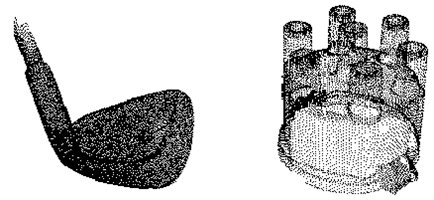
\includegraphics[scale=0.12]{images/CADCloud.png}
	\item Voxel 

	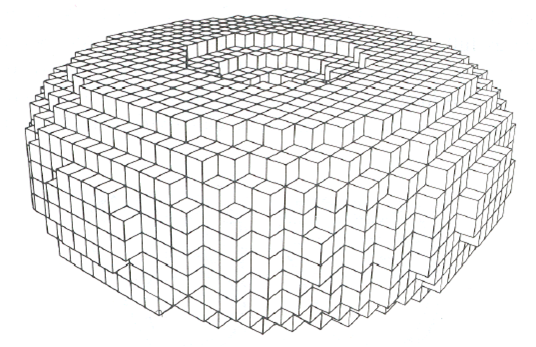
\includegraphics[scale=0.12]{images/CADVoxel.png}
	\item Mesh

	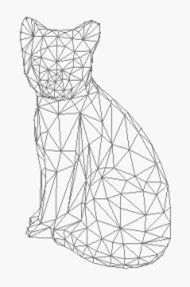
\includegraphics[scale=0.12]{images/CADMesh.png}
	\end{itemize}
\end{itemize}
\end{frame}


\begin{frame}{By Storage}
\begin{itemize}
\item Procedural model : CSG (Constructive Solid Geometry)

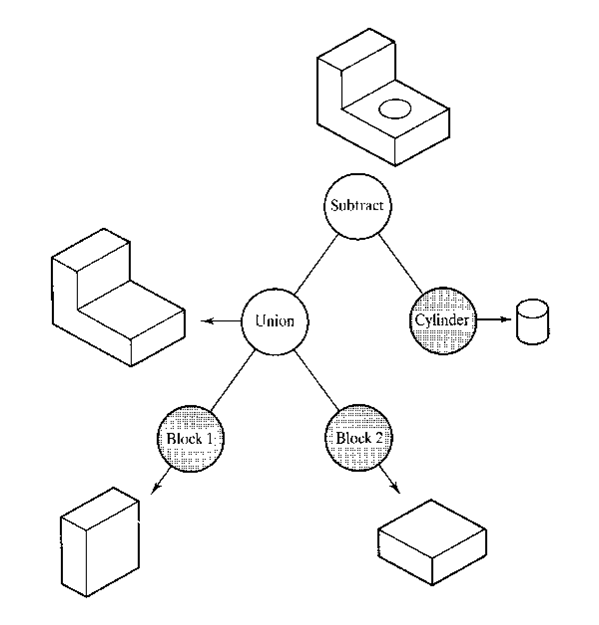
\includegraphics[scale=0.2]{images/CADCSG.png}
\item Result based model : B-Rep (Boundary representation)

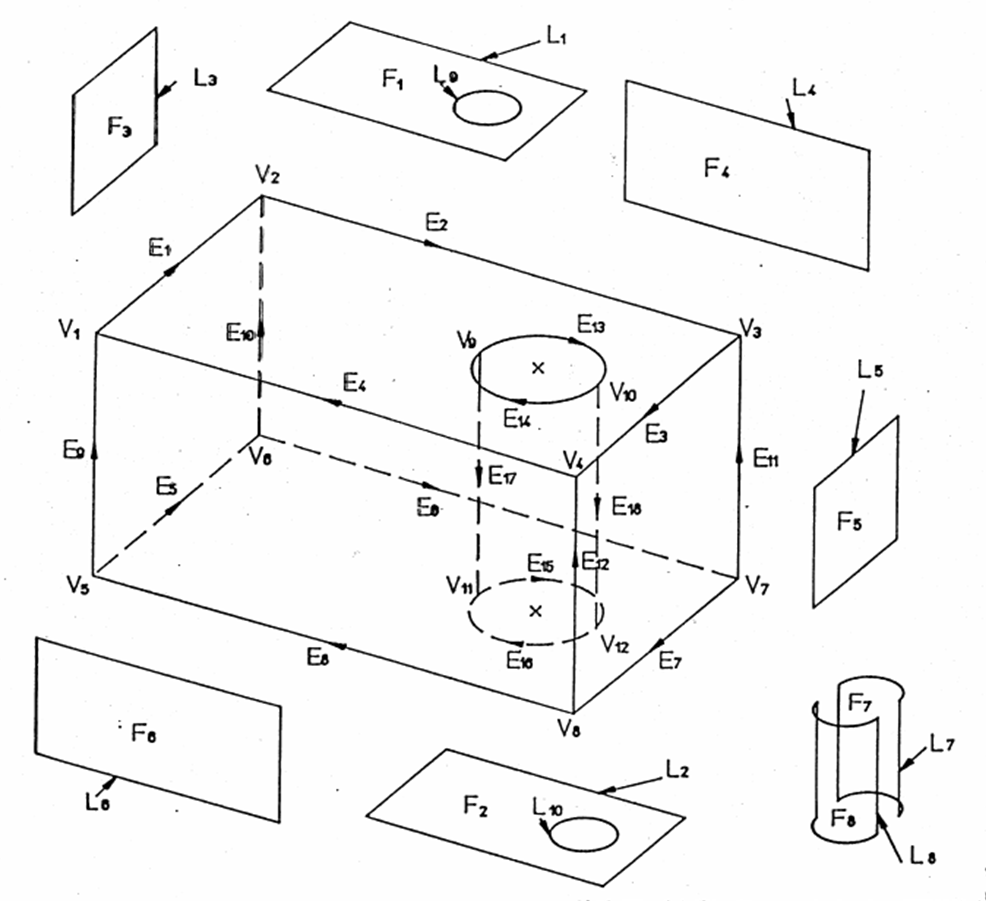
\includegraphics[scale=0.2]{images/CADBrep.png}
\end{itemize}
\end{frame}